\documentclass[]{report}
\renewcommand{\thesection}{\arabic{section}}
\usepackage{graphicx}


% Title Page
\title{Implementing neural networks with tensorflow report}
\author{Linus Edelkott, Tobias Petri}


\begin{document}
\maketitle

\begin{abstract}
The aim of this project is to create a virtual Texas Hold'em player by using a convolutional neural network, based on the paper "Poker-CNN: a pattern learning strategy for making draws and bets in poker games" \cite{1} by Yakovenko, Nikolai et. al.
The aim is to imitate human poker-playing behaviour, including bluffing, as close as possible - a task where current, non neural network based poker bots usually fail.
\end{abstract}


\section{Introduction}
Unlike other games such as chess or checkers, poker provides an especially challenging task for computer players (bots). That is because poker contains a very "human" component aside from its set of rules: the bidding, raising, the bluffing. Where other games only provide a reward upon successfully winning them, the reward itself is a key element of the poker turn structure. Furthermore, since Texas Hold'em poker can be played with up to 9 people at a regular game, the state space grows to an enormous size. All these factors lead to the fact that current bot implementations usually are rather weak. Confronted with a human player, these bots have the huge disadvantage of being predictable: They often show repetitive behaviour and are bad at bluffing [ CITATION NEEDED, genaue player anführen ]. Due to these barriers, the team of Yakovenko, Nikolai et. al. developed a CNN based approach that aims at surpassing the current implementations and even competing with human tournament players \cite{1}. As their data source, they used simple bots to generate a large training and validation set. Learning only from the successful games, the CNN should afterwards be easily able to surpass the weak bots.    

\section{The paper}
\subsection{Original}
\subsection{Our changes}
\section{The CNN architecture}

The convolutional neural network that was used within this project has an architecture similar to the original CNN from the paper\cite{1}. The input data is formatted as a 17x17x9 3-dimensional tensor, including all blablablubb [Wie zum Geier sieht denn nun unser Format eig. aus?]


\begin{figure}[h]
\caption{Network structure}
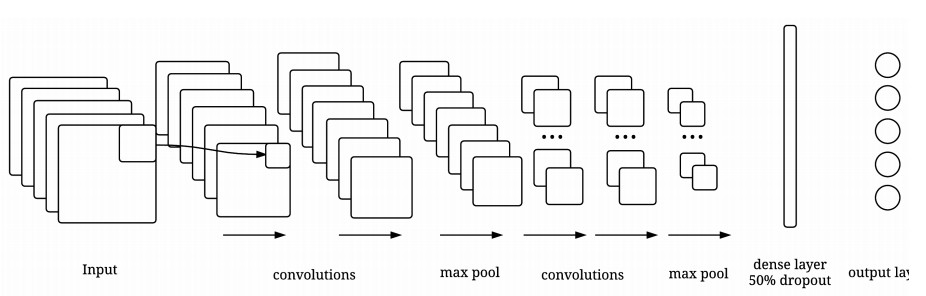
\includegraphics[scale = 0.5]{cnn_structure.jpg}
\end{figure}


\begin{thebibliography}{}
	\bibitem{1} Yakovenko, Nikolai, et al., \emph{Poker-CNN: a pattern learning strategy for making draws and bets in poker games}, arXiv preprint arXiv:1509.06731 (2015).
\end{thebibliography}  



\end{document}  

      
